\chapter{Theory}
\label{c:theory}

\section{Standard Model}

The standard model (SM) is a theory which describes the fundamental particles and their interactions. Matter consists of six quarks and six leptons, each of which has an anti-particle with opposite sign quantum numbers. They are organised into three generations each of which contains heavier particles than the last as seen in Table~\ref{table:SMmatter}. All of the stable matter of universe is made up of particles from the first generation. The leptonic sector consists of charged leptons, which can interact via the electromagnetic and weak forces, and neutrinos, which interact via the weak force. The neutrinos are assumed to be massless in the standard model however observations of neutrino oscillations revealed that neutrinos have mass.

\begin{table}[ht!]
\centering
\caption{Quarks and leptons}
\label{table:SMmatter}
\footnotesize
\begin{tabular}{|c|l|l|l|l|l|l|}
\hline
\multirow{2}{*}{Generation} & \multicolumn{3}{c|}{Quarks}                             & \multicolumn{3}{c|}{Leptons}              \\ \cline{2-7} 
                            & Flavour & Charge & Mass (MeV)                           & Flavour      & Charge & Mass (MeV)        \\ \hline
\hline

\multirow{2}{*}{I}          & u       & 2/3    & $2.2^{+0.6}_{-0.4}$                  & e            & -1     & 0.511             \\
                            & d       & -1/3   & $4.7^{+0.5}_{-0.4}$                  & $\nu_{e}$    & 0      & $<2\times10^{-6}$ \\ \hline
\multirow{2}{*}{II}         & c       & 2/3    & $(1.27\pm 0.03)\times10^{3}$         & $\mu$        & -1     & 105.66            \\
                            & s       & -1/3   & $96^{+8}_{-4}$                       & $\nu_{\mu}$  & 0      & $<0.19$           \\ \hline
\multirow{2}{*}{III}        & t       & 2/3    & $(173.21\pm0.51\pm0.71)\times10^{3}$ & $\tau$       & -1     & $1776.86\pm0.12$  \\
                            & b       & -1/3   & $(4.18^{+0.04}_{-0.3})\times10^{3}$  & $\nu_{\tau}$ & 0      & $<18.2$           \\ \hline
\end{tabular}
\end{table}

Quarks interact via the electromagnetic or strong force. Each quarks carries a colour charge of red, green or blue, where all three colours combined give a colourless combination, or a colour and it's anti-colour can give a colourless combination. This theory of colour confinement means that quarks can only be found in bound states of baryons or mesons, respectively. 
The top quarks is the heaviest quark with a mass approximately equivalent to a lead nuclei. The top quark is the only quark which predominantly decays before it hadronises due to it's short lifetime of $5\times10^{-25}$~seconds. The main decay mode for top quarks is to a bottom quark and a W boson which occurs $95.6\pm3.4\%$ of the time.
Finally, the force carries consist of gauge bosons of integer spin, as seen in table~\ref{table:SMbosons}. Photons and Z bosons can mediate neutral electroweak interactions whereas W bosons can mediate charged electroweak interactions. The gluons mediate the strong interaction and occur with 8 different types of colour charge which will be described in section~\ref{subsec:QCD}. 
The Graviton is hypothesised to carry the gravitational force but there is as yet no evidence to support this hypothesis.
\begin{table}[ht!]
\centering
\caption{Gauge bosons}
\footnotesize
\label{table:SMbosons}
\begin{tabular}{|l|l|l|l|l|l|}
\hline
Gauge boson                       & Force           & Charge & Mass (GeV) & Spin & Range (m)  \\ \hline \hline
Photon ($\gamma$)                 & electromagnetic & 0      & 0          & 1    & $\infty$   \\ \hline
W$^{\pm}$                         & weak            & $\pm1$ &            & 1    & $10^{-18}$ \\ \hline
Z                                 & weak            & 0      &            & 1    & $10^{-18}$ \\ \hline
gluon                             & strong          & 0      & 0          & 1    & $10^{-15}$ \\ \hline
Graviton\footnote\{hypothesised\} & gravitational   & 0      & 0          & 2    & $\infty$   \\ \hline
\end{tabular}
\end{table}

The discovery of the Higgs boson in 2012 completed the standard model with an explanation to how the fundamental particles have mass via the electroweak symmetry breaking mechanism.

\subsection{Electroweak theory}

\subsubsection{QED}
\label{subsec:QED}

Figure~\ref{fig:QEDvertex} shows the fundamental QED vertex where a charged particle (charged lepton or quark) and charged anti-particle interact with a photon. The convention in this thesis is that time flows from left to right. However, these diagrams may be rotated as long as they conserve energy. Hence, this diagram includes electron-positron annihilation into a photon, a photon pair-producing an electron-positron pair, an electron emitting a photon or a positron emitting a photon depending on the orientation of the diagram and assuming that the charged particles are first generation charged leptons. 

\begin{figure}[ht!]
\begin{center}
    \includegraphics[width=0.35\textwidth]{images/Theory/QEDvertex.png}
    \caption{Fundamental QED vertex}
    \label{fig:QEDvertex}
\end{center}
\end{figure}

This diagram alone cannot occur as it violates conservation of energy but can be used to build a full Feynman diagram for a particle physics process. QED interactions conserve lepton or quark flavour. 
The QED Lagrangian can be found in Eq.~\ref{eqn:QEDL} where $D_{\mu}$ represents the covariant derivative which is defined as X. 
\begin{equation}
\mathcal{L} = \overline{\phi}\left(i\gamma^{\mu}D_{\mu}-m\right)\phi - \frac{1}{4}F_{\mu\nu}F^{\mu\nu}
\label{eqn:QEDL}
\end{equation}
This Lagrangian is gauge invariant, ie. it is invariant under U(1) phase transformations, where U(1) is the unitary group.

\subsubsection{Weak interactions}

\begin{figure}[ht!]
\begin{center}
    \includegraphics[width=0.35\textwidth]{images/Theory/weakDecay.png}
    \caption{Proo}
    \label{fig:QEDvertex}
\end{center}
\end{figure}

\subsection{Quantum chromodynamics}
\label{subsec:QCD}
\begin{figure}[ht!]
\begin{center}
    \includegraphics[width=0.35\textwidth]{images/Theory/QCDvertex.png}
    \caption{Fundamental QCD vertex}
    \label{fig:QCDvertex}
\end{center}
\end{figure}



\section{Proton-proton collisions}

\section{Four top quark production}

The production of four top quarks occurs predominantly via gluon fusion, as seen at leading order in Fig.~\ref{fig:ttttAtLO}~(left), with a $10\%$ contribution from quark-anti-quark annihilation. The production mechanism occurs via QCD whereas the decay of top quarks via W bosons is a weak interaction. 

\begin{figure}[ht!]
\begin{center}
    \includegraphics[width=0.49\textwidth]{images/Theory/tttt_t_LO.pdf}
    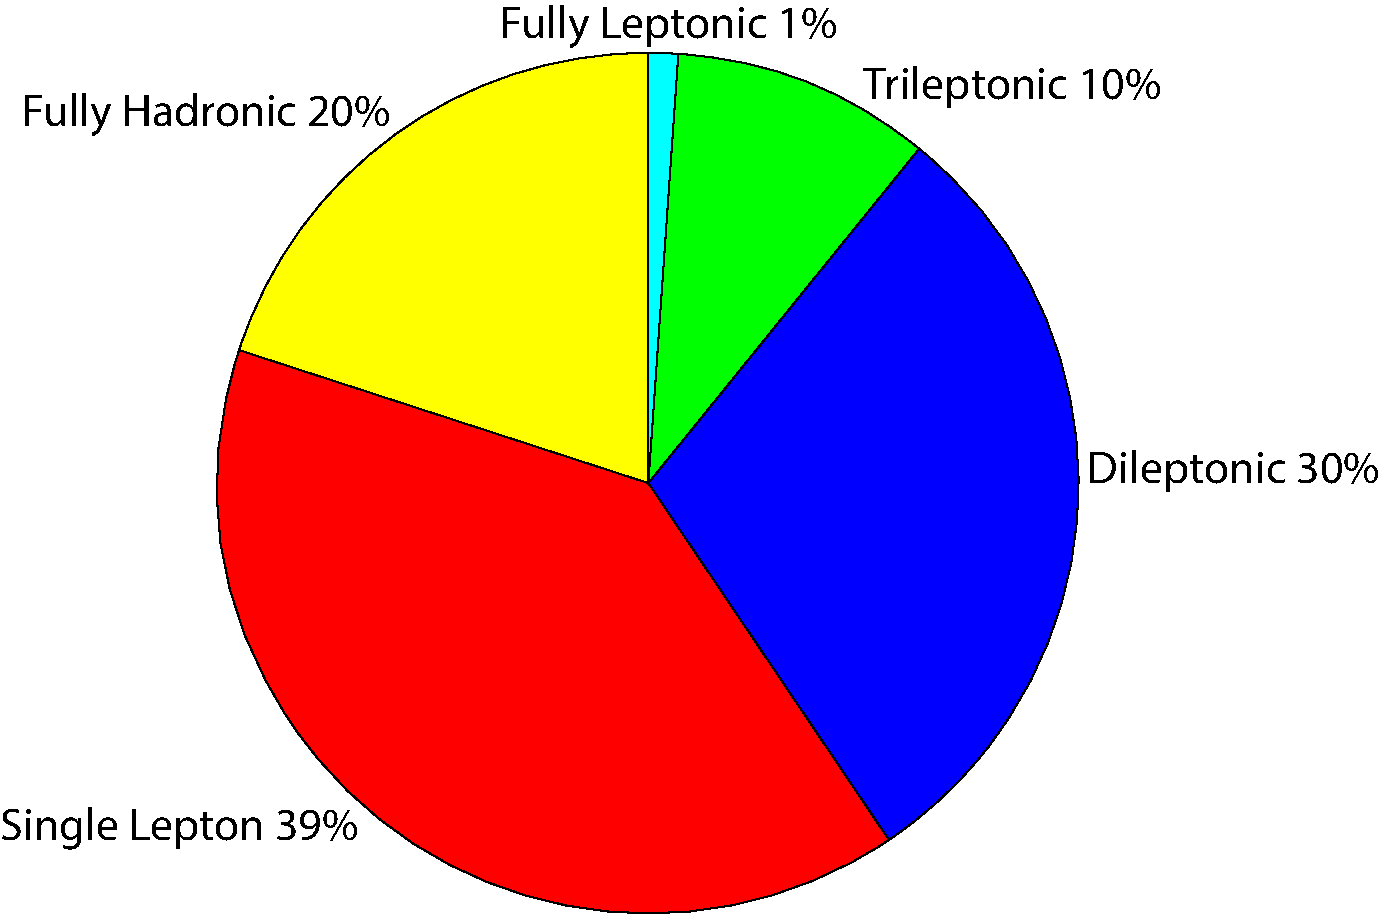
\includegraphics[width=0.4\textwidth]{images/Theory/FourTopBR.pdf}
    \caption{Dominant production mechanism for four top quarks in the standard model (left) and branching ratios for final states as defined by leptonic decays (right).}
    \label{fig:ttttAtLO}
\end{center}
\end{figure}

Final states are determined by the decay of the W boson which can occur either leptonically or hadronically as seen in Fig.~\ref{fig:topdecay}. It can be seen from Fig.~\ref{fig:ttttAtLO}~(right) that the single lepton final state has the largest branching ratio which makes a favourable place to look to study the largest number of events produced in the CMS detector. This is the final state considered most in this thesis. The dilepton final state also has a large branching ratio and has particularly low backgrounds when same-sign lepton final states are considered. The combination of studies on the dilepton final state will be discussed in the Chapter~\ref{c:Run2}.

\begin{figure}[ht!]
\begin{center}
    \includegraphics[width=0.55\textwidth]{images/Theory/topdecay.png}
    \caption{Top quark decay to a W boson and b-quark with subsequent decay of the W boson either leptonically or hadronically.}
    \label{fig:topdecay}
\end{center}
\end{figure}

\subsection{\ttbar background}

\subsection{Electroweak backgrounds}

\subsection{Rarer backgrounds}

\section{Shortcomings in the standard model}

\section{BSM models with four top quark signatures}



